\documentclass[a4paper,10pt,titlepage]{report}
\usepackage[utf8]{inputenc}
\usepackage[T1]{fontenc}
\usepackage[english]{babel}
\usepackage{amssymb}
\usepackage{amsmath}
\usepackage{amsthm}
\usepackage{graphicx}
\usepackage{fancyhdr}
\usepackage{lastpage}
\usepackage{pgfplots}
\usepackage{listings}
\usepackage{algorithm}
\usepackage{algpseudocode}
\usepackage{wrapfig}
\usepackage[document]{ragged2e}
\usepackage[margin=1in]{geometry}
\usepackage{enumitem}
\usepackage{color}
\usepackage{datenumber}
\usepackage{venndiagram}
\usepackage{chngcntr}
\setdatetoday
\addtocounter{datenumber}{0} %date for delivery standard is today
\setdatebynumber{\thedatenumber}
\date{}
\setcounter{secnumdepth}{0}
\pagestyle{fancy}
\fancyhf{}


%lstlisting ting:
\definecolor{dkgreen}{rgb}{0,0.45,0}
\definecolor{gray}{rgb}{0.5,0.5,0.5}
\definecolor{mauve}{rgb}{0.30,0,0.30}
\lstset{frame=tb,
  language=C++,
  aboveskip=3mm,
  belowskip=3mm,
  showstringspaces=false,
  columns=flexible,
  basicstyle={\small\ttfamily},
  numbers=left,
  numberstyle=\footnotesize,
  keywordstyle=\color{dkgreen}\bfseries,
  commentstyle=\color{dkgreen},
  stringstyle=\color{mauve},
  frame=single,
  breaklines=true,
  breakatwhitespace=false
  tabsize=1
}
\renewcommand{\lstlistingname}{Code}

\newcommand{\Z}{\mathbb{Z}}
\lhead{Algorithms in Cheminformatics (DM840)}
\rhead{Ilona Benko}
\rfoot{Page  \thepage \, of \pageref{LastPage}}
\counterwithin*{equation}{section}


\title{DM840 - mand 1}
\begin{document}
\begin{titlepage}
\centering
    \vspace*{9\baselineskip}
    \huge
    \bfseries
    1. Mandatory Assignment \\
    \normalfont
    Ilona Benko \\
    Ilben18 \\
	\huge
    Algorithms in Cheminformatics (DM840)  \\
    Daniel Merkle \\[4\baselineskip]
    \normalfont
	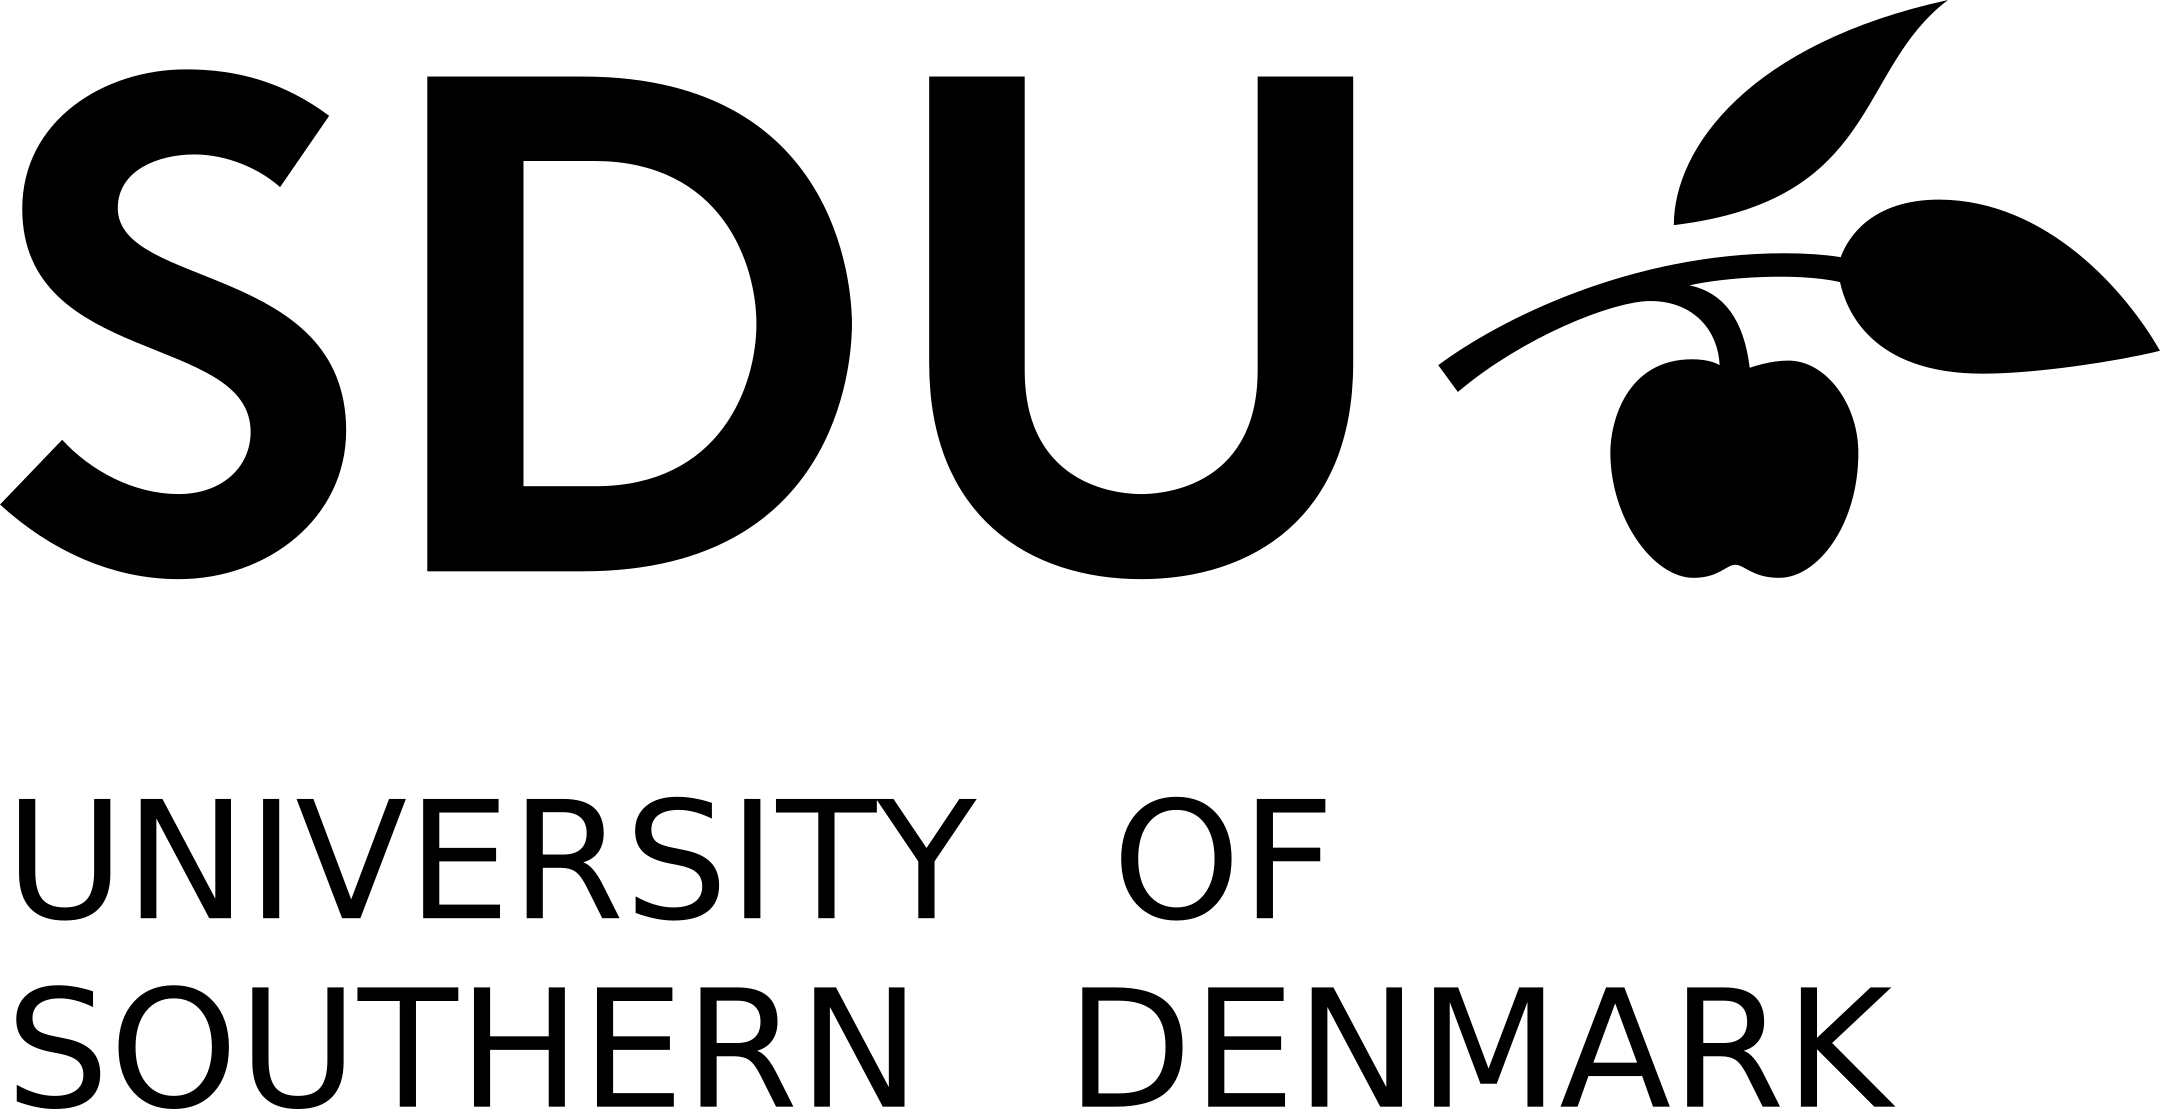
\includegraphics[scale=1]{SDU_logo}
    \vfill\
    \vspace{5mm}
    IMADA \\

    \textbf{\datedate}  \bf \\[2\baselineskip]
\end{titlepage}

\renewcommand{\thepage}{\roman{page}}% Roman numerals for page counter
\tableofcontents
\newpage
\setcounter{page}{1}
\renewcommand{\thepage}{\arabic{page}}
%https://www.overleaf.com/7644729885grfjqbyxxnbg

\section {Introduction}

The First assignment in the course contains 3 subparts, The Formose reaction, the Reindeer puzzle, and the Catalan game. The main aim of the assignment is to model these reactions and puzzles using graph grammars and to familiarize ourselves with MedØlDatschgerl software.
\newline
The formose reaction is one of the fundamental reactions in organic chemistry. Also, it's auto catalytic and therefore suitable for observing graph morphisms and applying double pushout approach. The two puzzles require more of the algorithmic approach.
\\
The Reindeer puzzle is situated in linear space which is divided to seven fields with two different types of reindeer. Three of each type are placed on each side and there is an empty field between them. The puzzle is considered solved when reindeer are transposed according to the movement restrictions.
\\
The Catalan game is based on graph contractions. Such contraction can occur if the observed vertex has exactly three attached edges. Each puzzle in the game is solved when the initial graph is contracted to a single node.
\\
Both of the puzzles can be abstracted and implemented in MØD by using graph grammars in the same manner as the chemical reactions and then solved using graph transformation rules. 
\\

\section{Design}
\subsection{Data formats}
\subsubsection{SMILES}
Smiles is a acronym for simplified molecular input line entry system that is used to express molecules in a string format and for this it uses a few operators. For bonds ., -, =, #, \$, :, / and \textbackslash can be used.
Rings are defined using numbers where you mark where a ring begins and ends, and these two points are connected. Within rings, they can be defined in three ways. One is using alternating single and double bonds, or using :, an example of this is  C1=CC=CC=C1 and C:1:C:C:C:C:C1 using the two different methods.
The third way is marking all the atoms in the ring using small letters.\\
Branches are defined using brackets, so a molecule may be represented as CCC(=O)C
Some other features that are supported are Stereochemistry and Isotopes. These weren't used to solve this assignment so won't be explained in this report.
\subsubsection{GML}
The Graph Modelling Language\cite{http://www.fim.uni-passau.de/fileadmin/files/lehrstuhl/brandenburg/projekte/gml/gml-technical-report.pdf} is defined using a Rule, it's defined as
\begin{equation}
    L \longleftarrow K \longrightarrow R
\end{equation}
constructed using three subgraphs, the left side, the context and the right side. From these we can generate L, R, and K they as defined as the following:
\begin{equation}
    L = left \cup Context
\end{equation}
\begin{equation}
    R as right \cup Context
\end{equation}
and
\begin{equation}
    K as context \cup (left \cap Right)
\end{equation}
left right, and context can include nodes and edges. Edges can be the glasses of the bonds mentioned above hand in the smiles notation. On the other hand, nodes can have a label and in some cases a charge. 
\subsection{MØD}
The MedØlDatschgerl is a graph-based cheminformatics Framework, but in this case, it was used to solve a game.
It takes GML-Rules and SMILES as an input and generates a report as an output. \\
The framework is accessed using a python API, and can also be used interactively using IPython.
\\
Furthermore, the platform has a built in ILP solver among other tools, so within the rules you can define constraints that are required to be met before a rule can be applied, which allows more complicated reactions to be done in a specific ordering if required.
\newpage
\section{Implementation and results}

The three subprojects where implemented using a skeleton code that was handed out with the project description. The skeleton code supplied consisted of the python API, and for some projects the .GML files with rule samples.
\subsection{Formose}
To complete the Formose reaction cycle, we needed to implement four rules and define SMILES string input of two molecules, Formaldehyde and Glycolaldehyde. The rules by which the Formose reaction can be completely described are Keto-enol isomerization and Aldol addition when applied in both directions. Those rules were defined using GML format.

\subsubsection{Formaldehyde and Glycolaldehyde}

There are numerous ways to represent nontrivial molecules using SMILES, in our implementation, we used C=O for Formaldehyde and O=CCO for Glycolaldehyde.

    \vspace{10mm}
    \hspace{50mm}
	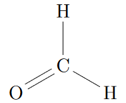
\includegraphics[scale=0.5]{fa}
	\hspace{15mm}
    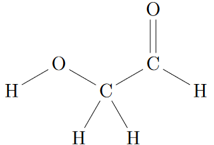
\includegraphics[scale=0.5]{ga}
    \vspace{10mm}
    
\subsubsection{Keto-enol isomerization}
The Keto-enol isomerization has to be used in both directions, forward and backwards, so this is expressed using two rules. 
In the forward reaction we have the transformation where O=CCH becomes C=COH.
This has to be defined as a graph grammar rule. 

Keto-enol forward:
\begin{lstlisting}
rule [
	ruleID "Keto-enol isomerization ->"
	left [
            edge [ source 1 target 2 label "-" ]
            edge [ source 2 target 3 label "=" ]
            edge [ source 1 target 4 label "-" ]
	]
	context [
            node [ id 1 label "C" ]
            node [ id 2 label "C" ]
            node [ id 3 label "O" ]
            node [ id 4 label "H" ]
	]
	right [
	    edge [ source 1 target 2 label "=" ]
            edge [ source 2 target 3 label "-" ]
            edge [ source 3 target 4 label "-" ]
	]
constrainAdj [
	    id 2
	    op "="
	    count 1
	    nodeLabels [ label "O" ]
	]
] 
\end{lstlisting}

As it follows, in backward reaction C=COH becomes O=CCH.
This also has to be defined as a graph grammar rule.  

Keto-enol backward:
\begin{lstlisting}
rule [
	ruleID "Keto-enol isomerization <-"
	left [
            edge [ source 1 target 2 label "=" ]
            edge [ source 2 target 3 label "-" ]
            edge [ source 3 target 4 label "-" ]
	]
	context [
            node [ id 1 label "C" ]
            node [ id 2 label "C" ]
            node [ id 3 label "O" ]
            node [ id 4 label "H" ]
	]
	right [
	    edge [ source 1 target 2 label "-" ]
            edge [ source 2 target 3 label "=" ]
            edge [ source 1 target 4 label "-" ]
	]
	constrainAdj [
	    id 2
	    op "-"
	    count 1
	    nodeLabels [ label "O" ]
	]
] 
\end{lstlisting}

This reaction is represented by MØD as a pushout diagram. 
\\
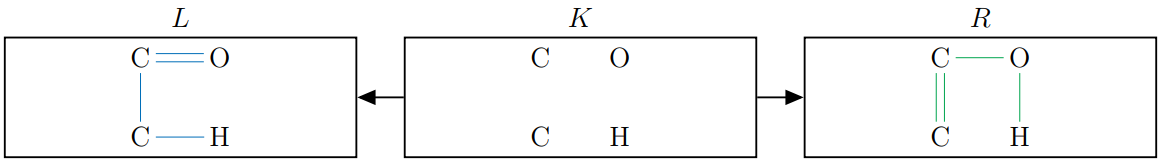
\includegraphics[scale= 0.5]{keto}

\subsubsection{Aldol-addtition}

The second reaction present in the Formose cycle is Aldol-addition. It also has to be used in both directions.

Aldol-addition forward:
\begin{lstlisting}
rule [
	ruleID "Aldol Addition ->"	
	left [
            edge [ source 1 target 2 label "=" ]
            edge [ source 2 target 3 label "-" ]
            edge [ source 3 target 4 label "-" ]
            edge [ source 5 target 6 label "=" ]
	]
	context [
            node [ id 1 label "C" ]
            node [ id 2 label "C" ]
            node [ id 3 label "O" ]
            node [ id 4 label "H" ]
            node [ id 5 label "O" ]
            node [ id 6 label "C" ]
	]
	right [
            edge [ source 1 target 2 label "-" ]
            edge [ source 2 target 3 label "=" ]
            edge [ source 4 target 5 label "-" ]
            edge [ source 5 target 6 label "-" ]
            edge [ source 6 target 1 label "-" ]
	]	
	constrainAdj [
	    id 2
	    op "="
	    count 1
	    nodeLabels [ label "O" ]
	]
	constrainAdj [
	    id 4
	    op "="
	    count 1
	    nodeLabels [ label "O" ]
	]
]

\end{lstlisting}

Aldol-addition backward:
\begin{lstlisting}
rule [
	ruleID "Aldol Addition <-"	
	left [
            edge [ source 1 target 2 label "-" ]
            edge [ source 2 target 3 label "=" ]
            edge [ source 4 target 5 label "-" ]
            edge [ source 5 target 6 label "-" ]
            edge [ source 6 target 1 label "-" ]
	]
	context [
            node [ id 1 label "C" ]
            node [ id 2 label "C" ]
            node [ id 3 label "O" ]
            node [ id 4 label "H" ]
            node [ id 5 label "O" ]
            node [ id 6 label "C" ]
	]
	right [
            edge [ source 1 target 2 label "=" ]
            edge [ source 2 target 3 label "-" ]
            edge [ source 3 target 4 label "-" ]
            edge [ source 5 target 6 label "=" ]
	]	
	constrainAdj [
	    id 2
	    op "="
	    count 1
	    nodeLabels [ label "O" ]
	]
	constrainAdj [
	    id 6
	    op "-"
	    count 1
	    nodeLabels [ label "O" ]
	]
]

\end{lstlisting}
This reaction is represented by MØD as a pushout diagram. 
\\
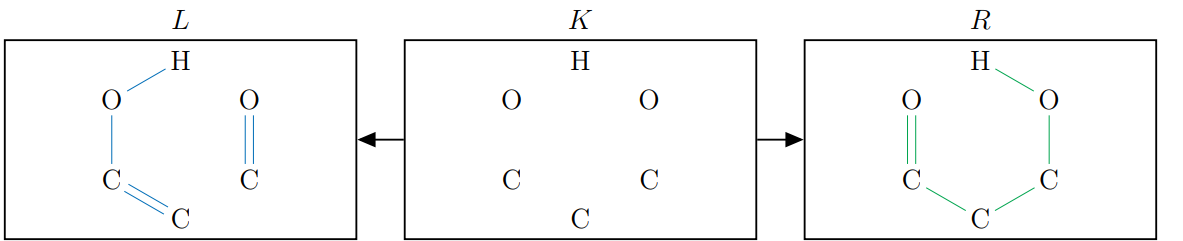
\includegraphics[scale= 0.5]{aldol}

When we expand our graph from our 3 starting molecules we get the following graph. \\
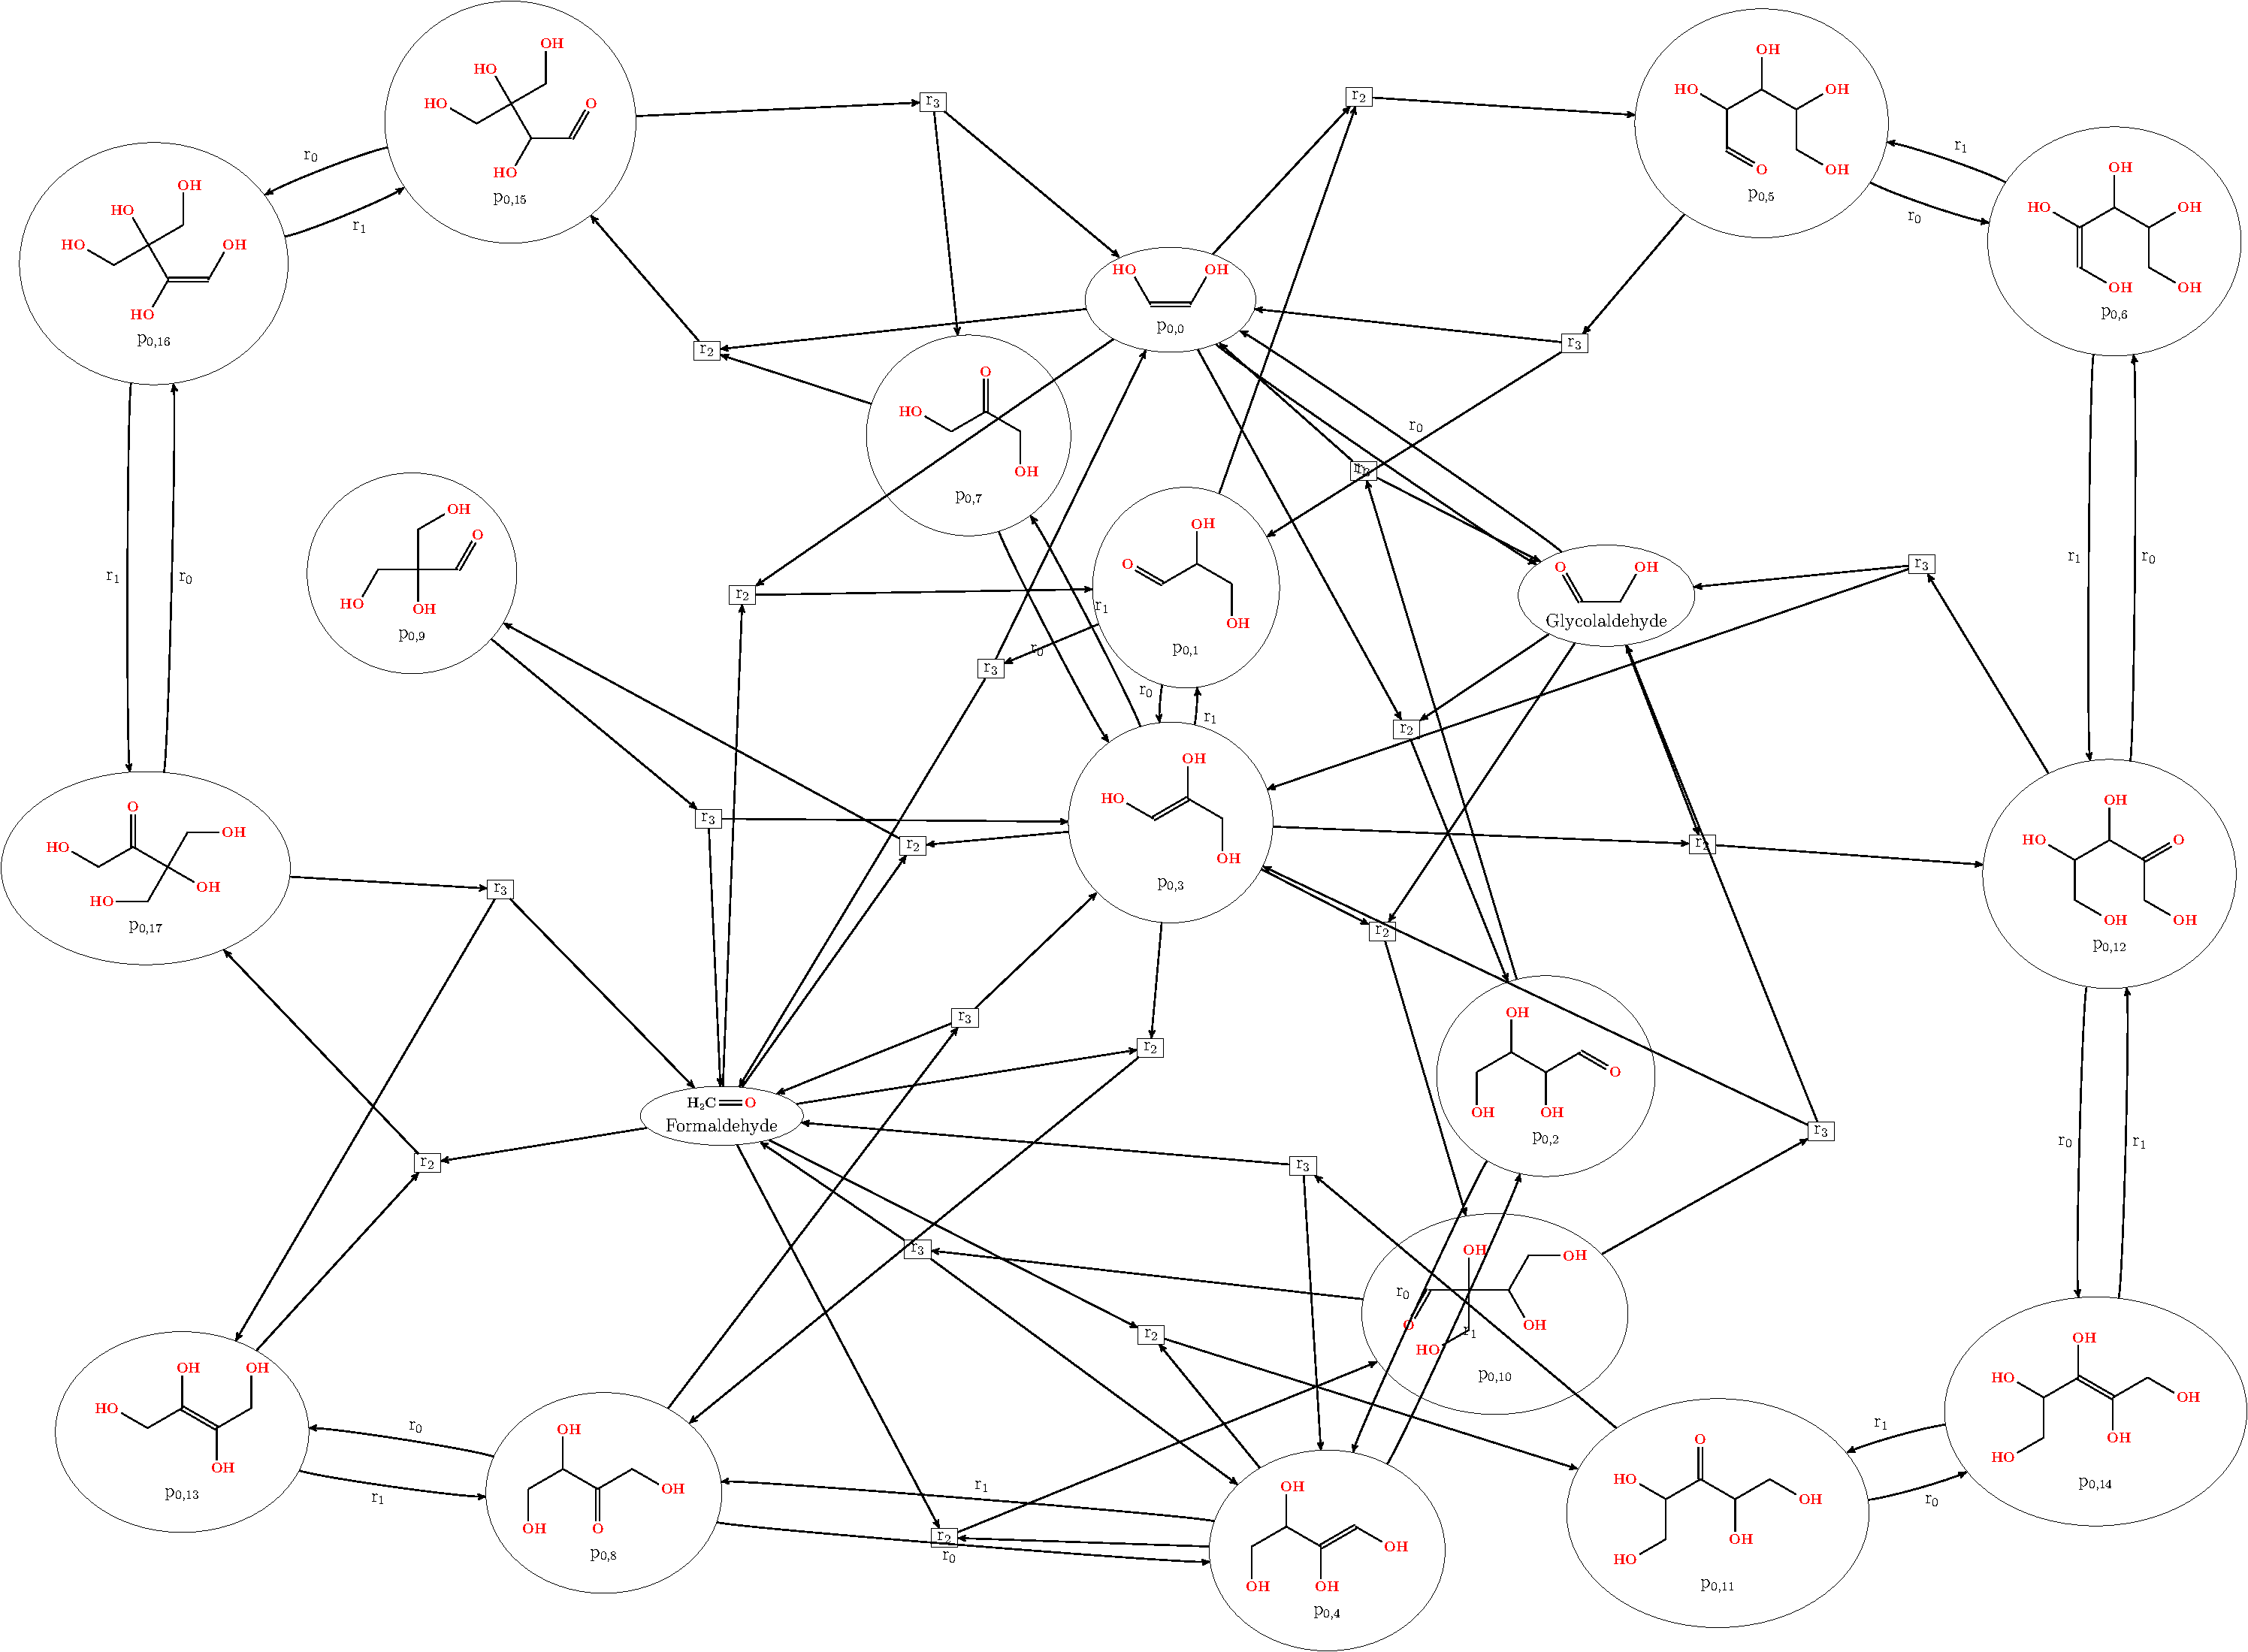
\includegraphics[width=1\textwidth, angle=0]{hyper.pdf}
\\
This graph is a map of all the possible deviations of our deviations of our reaction. and by doing a shortest path, or cheapest path from our starting molecules we get our filtered graph that shows the path from out input to out desired output, in this case 2 Glycolaldehyde molecules.
\\
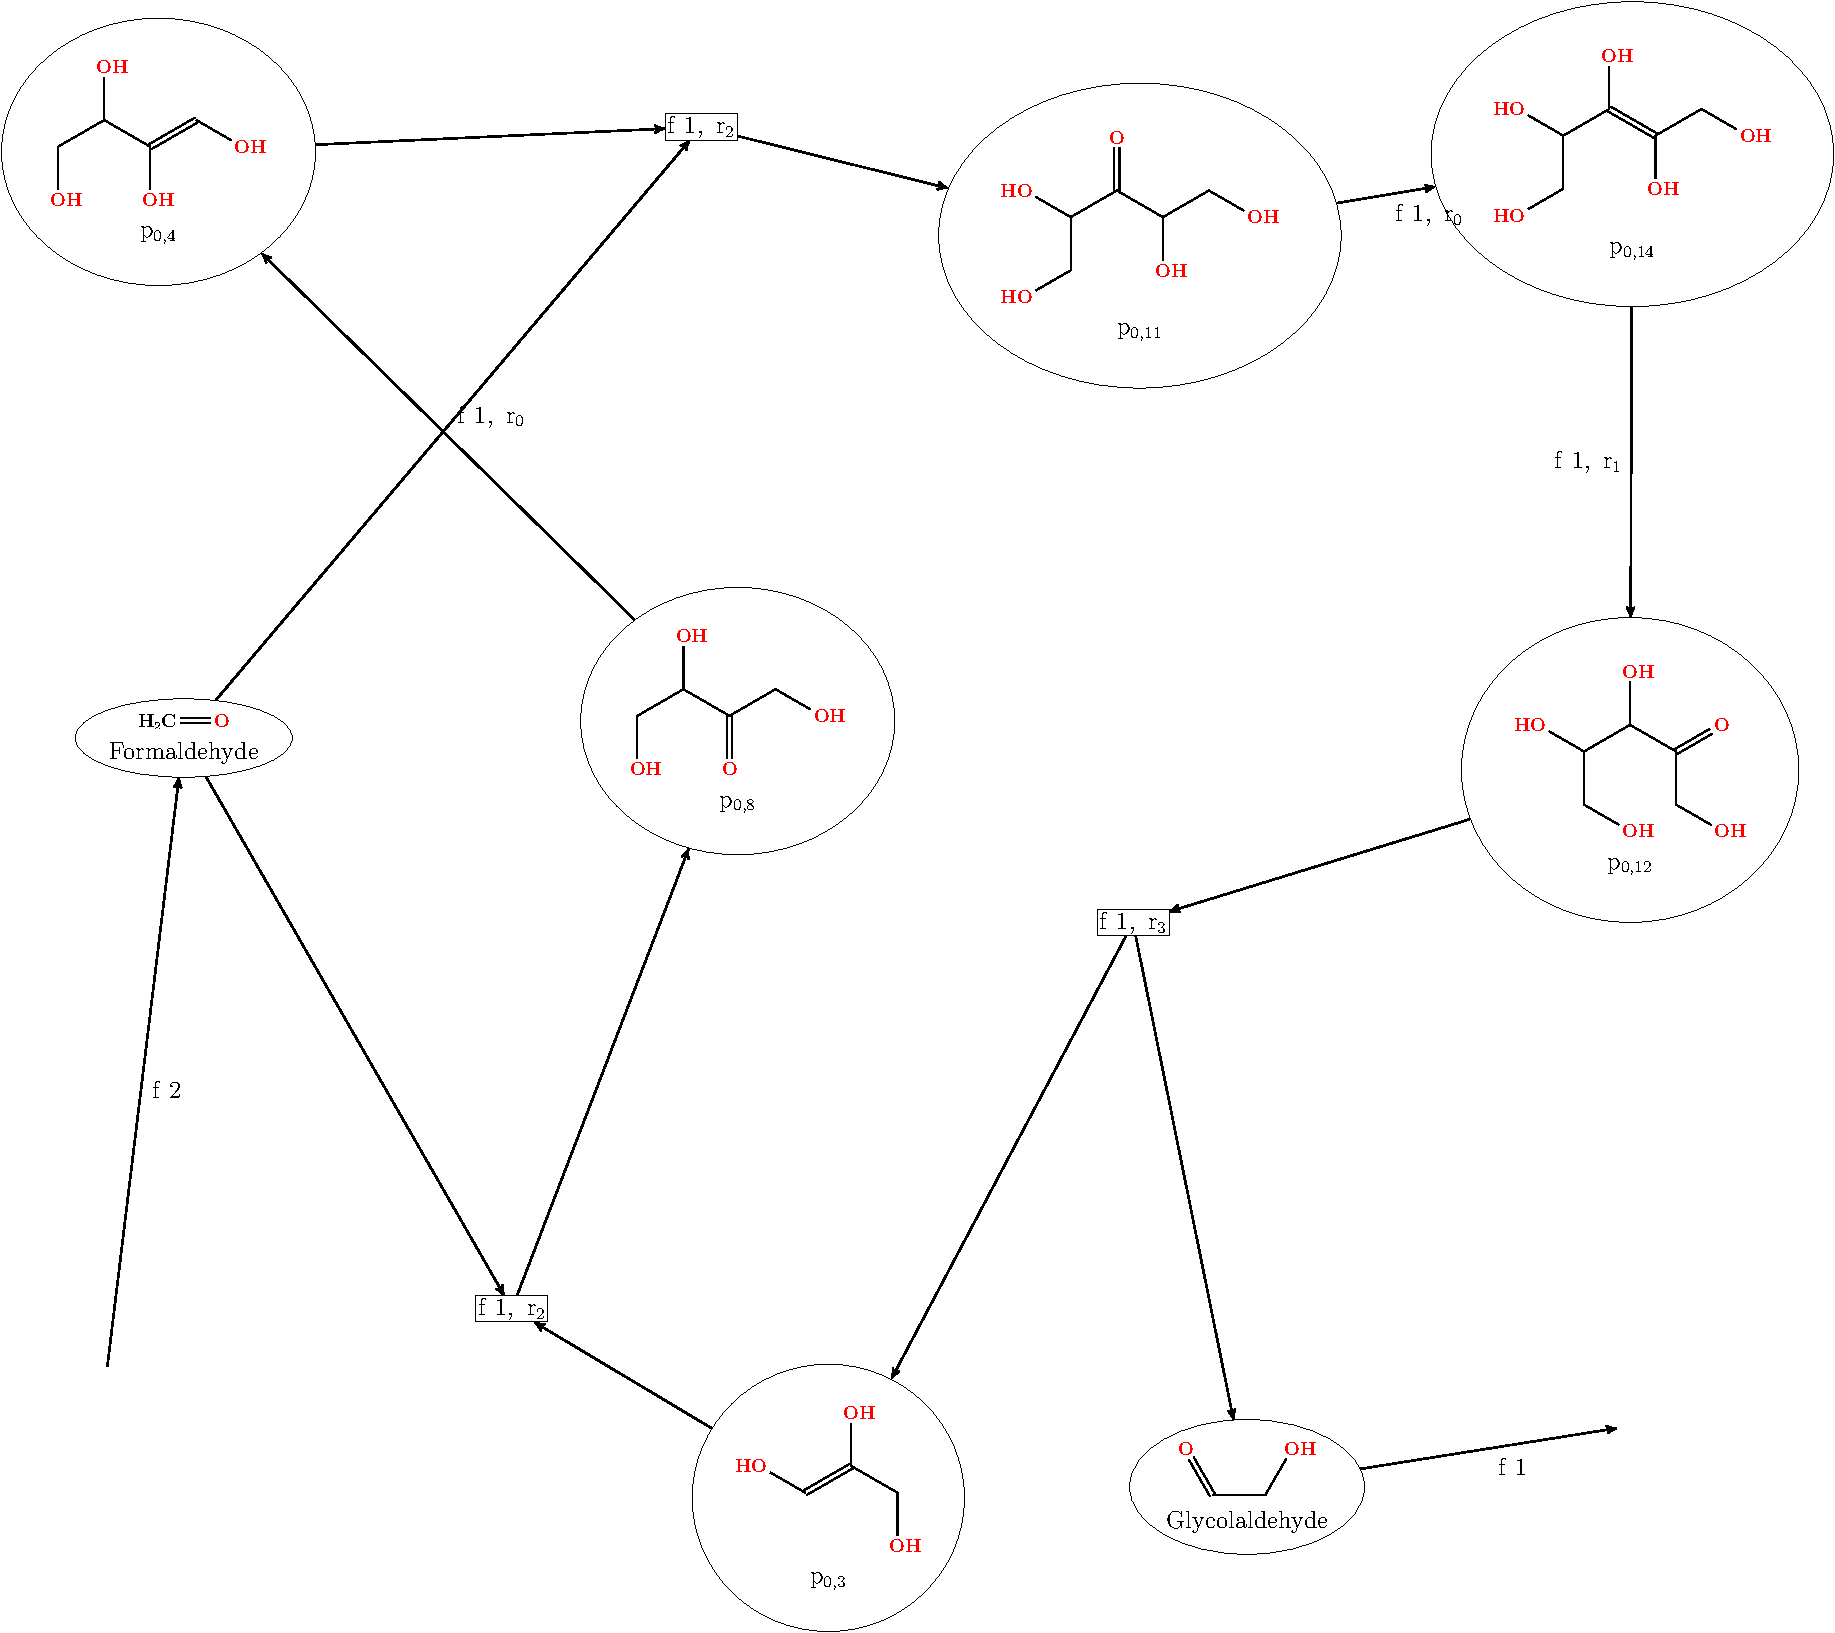
\includegraphics[width=0.5\textwidth, angle=0]{045.pdf}
\\
However, if you look at the diagram, this is not what is happening. It shows that when we're inputting 2 Formaldehyde we can get 1 Glycolaldehyde, but from the diagram we need a p0,3 to start the reaction and not the Glycolaldehyde as it should be.
\\
The objective value for the reaction is 0. which is odd, as it should be higher.

\subsection{Reindeer}

Reindeer puzzle required a different approach. The puzzle consists of six reindeer which can be moved linearly on seven different fields. The starting position's SMILES string is defined as: "SAAAEBBBT", where "S" represents the starting field, "T" the terminating field and "E" the blank field. "A" and "B" are reindeer of a different kinds. Goal is to reach terminating position defined as "TAAAEBBBS", in other terms, switch positions of the different kinds of reindeer. This has to be achieved by following two movement rules, jump and step. Step rule means that one reindeer is moving for one position and by that swapping position with blank position "E". Jump can happen only when reindeer of a one kind is positioned next to the reindeer of a different kind and next to that reindeer is blank position. In this terms, then the first reindeer and blank position swap places. 

To solve the puzzle, described rules had to be implemented in MØD using GML. As this is a pure algorithmic puzzle, we solved it on the paper in sixteen steps and then rewrote each step as a graph grammar rule. Each algorithm instance is imagined as a different molecule, where reindeer and additional strings represent atoms connected with single bonds. To transform one instance into another when following the "step" rule, we are changing the surroundings of four atoms and to define a "jump", five atoms have to be used. The complete solution consists of fourteen rules defined as follows:

\begin{lstlisting}
s = "SAAAEBBBT"
t = "TAAAEBBBS"

g = graphDFS("".join("[%s]" % a for a in s))
g.print()
goal = graphDFS("".join("[%s]" % a for a in t))
goal.print()

AAEBstep = ruleGMLString("""rule [
	ruleID "AAEB step"
	left [
        edge [ source 0 target 1 label "-" ]
        edge [ source 1 target 2 label "-" ]
        edge [ source 2 target 3 label "-" ]
	]
	context [
        node [ id 0 label "A" ]
        node [ id 1 label "A" ]
        node [ id 2 label "E" ]
        node [ id 3 label "B" ]
	]
	right [
        edge [ source 0 target 2 label "-" ]
        edge [ source 1 target 3 label "-" ]
        edge [ source 2 target 1 label "-" ]
	]
]""")

AEBBstep = ruleGMLString("""rule [
	ruleID "AEBB step"
	left [
        edge [ source 0 target 1 label "-" ]
        edge [ source 1 target 2 label "-" ]
        edge [ source 2 target 3 label "-" ]
	]
	context [
        node [ id 0 label "A" ]
        node [ id 1 label "E" ]
        node [ id 2 label "B" ]
        node [ id 3 label "B" ]
	]
	right [
        edge [ source 0 target 2 label "-" ]
        edge [ source 1 target 3 label "-" ]
        edge [ source 2 target 1 label "-" ]
	]
]""")

SAEBstep = ruleGMLString("""rule [
	ruleID "SAEB step"
	left [
        edge [ source 0 target 1 label "-" ]
        edge [ source 1 target 2 label "-" ]
        edge [ source 2 target 3 label "-" ]
	]
	context [
        node [ id 0 label "S" ]
        node [ id 1 label "A" ]
        node [ id 2 label "E" ]
        node [ id 3 label "B" ]
	]
	right [
        edge [ source 0 target 2 label "-" ]
        edge [ source 1 target 3 label "-" ]
        edge [ source 2 target 1 label "-" ]
	]
]""")

BAETstep = ruleGMLString("""rule [
	ruleID "AEBA step"
	left [
        edge [ source 0 target 1 label "-" ]
        edge [ source 1 target 2 label "-" ]
        edge [ source 2 target 3 label "-" ]
	]
	context [
        node [ id 0 label "B" ]
        node [ id 1 label "A" ]
        node [ id 2 label "E" ]
        node [ id 3 label "T" ]
	]
	right [
        edge [ source 0 target 2 label "-" ]
        edge [ source 1 target 3 label "-" ]
        edge [ source 2 target 1 label "-" ]
	]
]""")

BEBAstep = ruleGMLString("""rule [
	ruleID "AEBA step"
	left [
        edge [ source 0 target 1 label "-" ]
        edge [ source 1 target 2 label "-" ]
        edge [ source 2 target 3 label "-" ]
	]
	context [
        node [ id 0 label "B" ]
        node [ id 1 label "E" ]
        node [ id 2 label "B" ]
        node [ id 3 label "A" ]
	]
	right [
        edge [ source 0 target 2 label "-" ]
        edge [ source 1 target 3 label "-" ]
        edge [ source 2 target 1 label "-" ]
	]
]""")

BAEAstep = ruleGMLString("""rule [
	ruleID "AEBA step"
	left [
        edge [ source 0 target 1 label "-" ]
        edge [ source 1 target 2 label "-" ]
        edge [ source 2 target 3 label "-" ]
	]
	context [
        node [ id 0 label "B" ]
        node [ id 1 label "A" ]
        node [ id 2 label "E" ]
        node [ id 3 label "A" ]
	]
	right [
        edge [ source 0 target 2 label "-" ]
        edge [ source 1 target 3 label "-" ]
        edge [ source 2 target 1 label "-" ]
	]
]""")

AEABBjump = ruleGMLString("""rule [
	ruleID "AEABB Jump"
	left [
        edge [ source 0 target 1 label "-" ]
        edge [ source 1 target 2 label "-" ]
        edge [ source 2 target 3 label "-" ]
        edge [ source 3 target 4 label "-" ]
	]
	context [
        node [ id 0 label "A" ]
        node [ id 1 label "E" ]
        node [ id 2 label "A" ]
        node [ id 3 label "B" ]
        node [ id 4 label "B" ]
	]
	right [
        edge [ source 0 target 3 label "-" ]
        edge [ source 1 target 4 label "-" ]
        edge [ source 2 target 1 label "-" ]
        edge [ source 3 target 2 label "-" ]
	]
]""")

BABEBjump = ruleGMLString("""rule [
	ruleID "BABEB Jump"
	left [
        edge [ source 0 target 1 label "-" ]
        edge [ source 1 target 2 label "-" ]
        edge [ source 2 target 3 label "-" ]
        edge [ source 3 target 4 label "-" ]
	]
	context [
        node [ id 0 label "B" ]
        node [ id 1 label "A" ]
        node [ id 2 label "B" ]
        node [ id 3 label "E" ]
        node [ id 4 label "B" ]
	]
	right [
        edge [ source 0 target 3 label "-" ]
        edge [ source 1 target 4 label "-" ]
        edge [ source 2 target 1 label "-" ]
        edge [ source 3 target 2 label "-" ]
	]
]""")

AABEBjump = ruleGMLString("""rule [
	ruleID "AABEB Jump"
	left [
        edge [ source 0 target 1 label "-" ]
        edge [ source 1 target 2 label "-" ]
        edge [ source 2 target 3 label "-" ]
        edge [ source 3 target 4 label "-" ]
	]
	context [
        node [ id 0 label "A" ]
        node [ id 1 label "A" ]
        node [ id 2 label "B" ]
        node [ id 3 label "E" ]
        node [ id 4 label "B" ]
	]
	right [
        edge [ source 0 target 3 label "-" ]
        edge [ source 1 target 4 label "-" ]
        edge [ source 2 target 1 label "-" ]
        edge [ source 3 target 2 label "-" ]
	]
]""")

SEABAjump = ruleGMLString("""rule [
	ruleID "SEABA Jump"
	left [
        edge [ source 0 target 1 label "-" ]
        edge [ source 1 target 2 label "-" ]
        edge [ source 2 target 3 label "-" ]
        edge [ source 3 target 4 label "-" ]
	]
	context [
        node [ id 0 label "S" ]
        node [ id 1 label "E" ]
        node [ id 2 label "A" ]
        node [ id 3 label "B" ]
        node [ id 4 label "A" ]
	]
	right [
        edge [ source 0 target 3 label "-" ]
        edge [ source 1 target 4 label "-" ]
        edge [ source 2 target 1 label "-" ]
        edge [ source 3 target 2 label "-" ]
	]
]""")

AEABAjump = ruleGMLString("""rule [
	ruleID "AEABA Jump"
	left [
        edge [ source 0 target 1 label "-" ]
        edge [ source 1 target 2 label "-" ]
        edge [ source 2 target 3 label "-" ]
        edge [ source 3 target 4 label "-" ]
	]
	context [
        node [ id 0 label "A" ]
        node [ id 1 label "E" ]
        node [ id 2 label "A" ]
        node [ id 3 label "B" ]
        node [ id 4 label "A" ]
	]
	right [
        edge [ source 0 target 3 label "-" ]
        edge [ source 1 target 4 label "-" ]
        edge [ source 2 target 1 label "-" ]
        edge [ source 3 target 2 label "-" ]
	]
]""")

AEABTjump = ruleGMLString("""rule [
	ruleID "AEABT Jump"
	left [
        edge [ source 0 target 1 label "-" ]
        edge [ source 1 target 2 label "-" ]
        edge [ source 2 target 3 label "-" ]
        edge [ source 3 target 4 label "-" ]
	]
	context [
        node [ id 0 label "A" ]
        node [ id 1 label "E" ]
        node [ id 2 label "A" ]
        node [ id 3 label "B" ]
        node [ id 4 label "T" ]
	]
	right [
        edge [ source 0 target 3 label "-" ]
        edge [ source 1 target 4 label "-" ]
        edge [ source 2 target 1 label "-" ]
        edge [ source 3 target 2 label "-" ]
	]
]""")

BABEAjump = ruleGMLString("""rule [
	ruleID "BABEA Jump"
	left [
        edge [ source 0 target 1 label "-" ]
        edge [ source 1 target 2 label "-" ]
        edge [ source 2 target 3 label "-" ]
        edge [ source 3 target 4 label "-" ]
	]
	context [
        node [ id 0 label "B" ]
        node [ id 1 label "A" ]
        node [ id 2 label "B" ]
        node [ id 3 label "E" ]
        node [ id 4 label "A" ]
	]
	right [
        edge [ source 0 target 3 label "-" ]
        edge [ source 1 target 4 label "-" ]
        edge [ source 2 target 1 label "-" ]
        edge [ source 3 target 2 label "-" ]
	]
]""")

BEABAjump = ruleGMLString("""rule [
	ruleID "BABEA Jump"
	left [
        edge [ source 0 target 1 label "-" ]
        edge [ source 1 target 2 label "-" ]
        edge [ source 2 target 3 label "-" ]
        edge [ source 3 target 4 label "-" ]
	]
	context [
        node [ id 0 label "B" ]
        node [ id 1 label "E" ]
        node [ id 2 label "A" ]
        node [ id 3 label "B" ]
        node [ id 4 label "A" ]
	]
	right [
        edge [ source 0 target 3 label "-" ]
        edge [ source 1 target 4 label "-" ]
        edge [ source 2 target 1 label "-" ]
        edge [ source 3 target 2 label "-" ]
	]
]""")
\end{lstlisting}

Represented above is the "brute-force" solution. Puzzle could be solved in a much simple way using wild cards. In that case, only four rules are needed, two to define stepping forwards for A and B and two for jumping: 

\begin{lstlisting}
aJump = ruleGMLString("""rule [
  ruleID "A Jump"
 	left [
         edge [ source 0 target 1 label "-" ]
         edge [ source 1 target 2 label "-" ]
         edge [ source 2 target 3 label "-" ]
         edge [ source 3 target 4 label "-" ]
 	]
 	context [
         node [ id 0 label "*" ]
         node [ id 1 label "A" ]
         node [ id 2 label "B" ]
         node [ id 3 label "E" ]
         node [ id 4 label "*" ]
 	]
 	right [
         edge [ source 0 target 3 label "-" ]
         edge [ source 1 target 4 label "-" ]
         edge [ source 2 target 1 label "-" ]
         edge [ source 3 target 2 label "-" ]
 	]
 ]""")

bJump = ruleGMLString("""rule [
 	ruleID "B Jump"
 	left [
         edge [ source 0 target 1 label "-" ]
         edge [ source 1 target 2 label "-" ]
         edge [ source 2 target 3 label "-" ]
         edge [ source 3 target 4 label "-" ]
 	]
 	context [
         node [ id 0 label "*" ]
         node [ id 1 label "E" ]
         node [ id 2 label "A" ]
         node [ id 3 label "B" ]
         node [ id 4 label "*" ]
 	]
 	right [
         edge [ source 0 target 3 label "-" ]
         edge [ source 1 target 4 label "-" ]
         edge [ source 2 target 1 label "-" ]
         edge [ source 3 target 2 label "-" ]
 	]
 ]""")

aStep = ruleGMLString("""rule [
 	ruleID "A step"
 	left [
 	 edge [ source 0 target 1 label "-" ]
         edge [ source 2 target 3 label "-" ]
 	]
 	context [
         node [ id 0 label "*" ]
         node [ id 1 label "A" ]
         edge [ source 1 target 2 label "-" ]
         node [ id 2 label "E" ]
         node [ id 3 label "*" ]
 	]
 	right [
 	 edge [ source 0 target 2 label "-" ]
         edge [ source 1 target 3 label "-" ]
 	]
 ]""")

bStep = ruleGMLString("""rule [
 	ruleID "B step"
 	left [
 	 edge [ source 0 target 1 label "-" ]
         edge [ source 2 target 3 label "-" ]
 	]
 	context [
         node [ id 0 label "*" ]
         node [ id 1 label "B" ]
         edge [ source 1 target 2 label "-" ]
         node [ id 2 label "E" ]
         node [ id 3 label "*" ]
 	]
 	right [
 	 edge [ source 0 target 2 label "-" ]
         edge [ source 1 target 3 label "-" ]
 	]
 ]""")

\end{lstlisting}

\newpage

\subsection{Catalan}

We implemented the total of six rules whose titles we got with the skeleton code to solve the Catalan puzzle. Those six rules combined and applied upon graphs simulate the Catalan game. In the game, the goal is to contract vertices which have exactly three neighbours so we end up with only one vertex. Different solutions can be obtained based on the order vertices are picked. Not all of them are valid. In this assignment graph grammars and algorithmic approach were applied by creating six universal rules which lead to correct solution for all 56 Catalan levels. 

\subsubsection{I. Mark for conversion}

This rule chooses the vertex which has three neighbours and marks it with "A" so it could be 'contracted' afterwards. Neighbouring vertices are marked with "R". Starting state is shown in the left part where all vertices in the graph are marked with "0". The most important part of this rule to work correctly are the five added constraints. The first two define the valid central node and the last three connection to the neighbouring nodes. \\
However, those constraints weren't enough because there could still be situations where there are many different vertices to which this rule could be applied. This is not desirable as we should have only one vertex marked for contraction at the same time, so we added a global constraint to stop this from happening. 

\begin{lstlisting}
rule [
	ruleID "Mark for conversion"
	left [
		node [ id 0 label "0" ]
		node [ id 1 label "0" ]
		node [ id 2 label "0" ]
		node [ id 3 label "0" ]
	]
	context [
		edge [ source 0 target 1 label "-" ]
		edge [ source 0 target 2 label "-" ]
		edge [ source 0 target 3 label "-" ]
	]
	right [
		node [ id 0 label "A" ]
		node [ id 1 label "R" ]
		node [ id 2 label "R" ]
		node [ id 3 label "R" ]
	]
	constrainAdj [
        id 0
		op "="
		count 0
		nodeLabels [ label "A" ]
	]
	constrainAdj [
		id 0
		op "="
		count 3
		nodeLabels [ label "0" ]
	]
	constrainAdj [
		id 1
		op "="
		count 0
		nodeLabels [ label "A" label "R" ]
	]
	constrainAdj [
		id 2
		op "="
		count 0
		nodeLabels [ label "A" label "R" ]
	]
	constrainAdj [
		id 3
		op "="
		count 0
		nodeLabels [ label "A" label "R" ]
	]
]
\end{lstlisting}

\vspace{10mm}
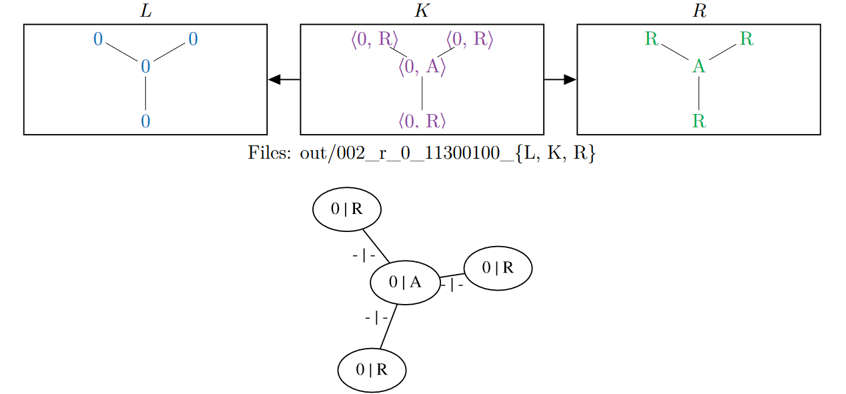
\includegraphics[scale=0.7]{i}
\vspace{10mm}

\subsubsection{II. Reattach external edge}

As the title states, this rule takes the edge which is connecting external edge  R-0 and as a result returns A-0, so outer node is being attached to the central node A instead of internal node R. This happens to all three neighbours because we have declared that type of connection in the context. In the end, we have the central node A which is connected to three neighbouring Rs, internal nodes and three 0s. The edges which were connecting Rs to 0s are deleted and replaced by the edges connecting A to 0s. No extra constraints were needed as there is only one A node and rule should be applied to all neighbours of A. 

\begin{lstlisting}
rule [
	ruleID "Reattach external edge"
	left [
		edge [ source 1 target 2 label "-" ]
	]
	context [
		edge [ source 0 target 1 label "-" ]
	        node [ id 0 label "A" ]
		node [ id 1 label "R" ]
		node [ id 2 label "0" ]
	]
	right [
	        edge [ source 0 target 2 label "-" ]
	]
]
\end{lstlisting}

\vspace{10mm}
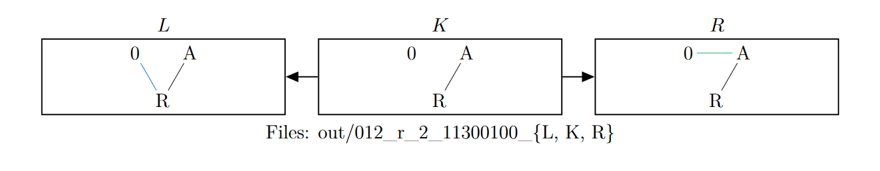
\includegraphics[scale=0.7]{ii_1.png}

\includegraphics[scale=0.7]{ii_2.png}
\vspace{10mm}

\subsubsection{III. Remove already attached}

The central thing which remains the same in the context is node A. This rule is used to delete internal nodes and edges marked by R in the first rule as they disappear while contraction is happening. It is safe to do so as we have connected external nodes marked by 0 to the central node by applying rule II. 

\begin{lstlisting}
rule [
	ruleID "Remove already attached"
	left [
		node [ id 1 label "R" ]
		node [ id 2 label "R" ]
		node [ id 3 label "R" ]
		edge [ source 0 target 1 label "-" ]
		edge [ source 0 target 2 label "-" ]
		edge [ source 0 target 3 label "-" ]
	]
	context [
                node [ id 0 label "A" ]
	]
	right [
	]
]
\end{lstlisting}

\vspace{10mm}
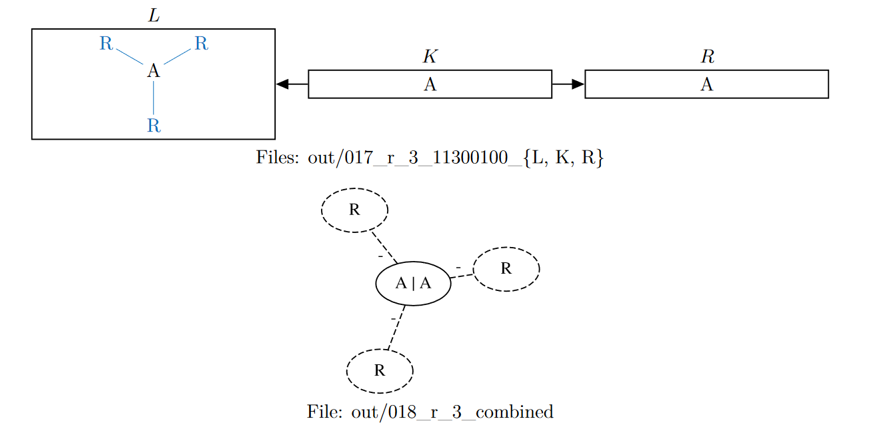
\includegraphics[scale=0.7]{iii.png}
\vspace{10mm}

\subsubsection{IV. Remove internal edge}

This rule is used to delete edges which are connecting two nodes marked with R if such exist, as they also disappear while contraction is happening. On the left side of the rule we declare the edge which is connecting two Rs and in the context we also need to describe how are those nodes 'related' to A as there could be cases when not all three neighbouring nodes R are connected internally.

\begin{lstlisting}
rule [
	ruleID "Remove internal edge"
	left [
		edge [ source 1 target 2 label "-" ]
	]
	context [
		node [ id 0 label "A" ]
		node [ id 1 label "R" ]
		node [ id 2 label "R" ]
		edge [ source 0 target 1 label "-" ]
		edge [ source 0 target 2 label "-" ]
	]
	right [
	]
]
\end{lstlisting}

\vspace{10mm}
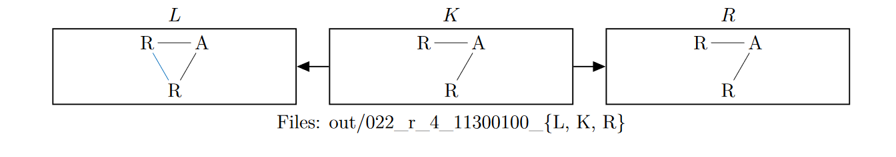
\includegraphics[scale=0.7]{iv_1.png}

\includegraphics[scale=0.7]{iv_2.png}
\vspace{10mm}

\subsubsection{V. Remove external edge}

Remove external edge deletes the bonds between internal and external neighbouring nodes, Rs and 0s. It is needed because after we connected 0s to A and deleted internal nodes Rs and edges connecting them to A, there may still be bonds which were connecting outer nodes 0s and Rs which are no longer needed as the other node which they were connecting is deleted and 0s are connected to A. 

\begin{lstlisting}
rule [
	ruleID "Remove external edge"
	left [
		edge [ source 1 target 2 label "-" ]
	]
	context [
		edge [ source 0 target 1 label "-" ]
		edge [ source 0 target 2 label "-" ]
	    node [ id 0 label "A" ]
		node [ id 1 label "R" ]
		node [ id 2 label "0" ]
	]
	right [
	]

]
\end{lstlisting}

\vspace{10mm}
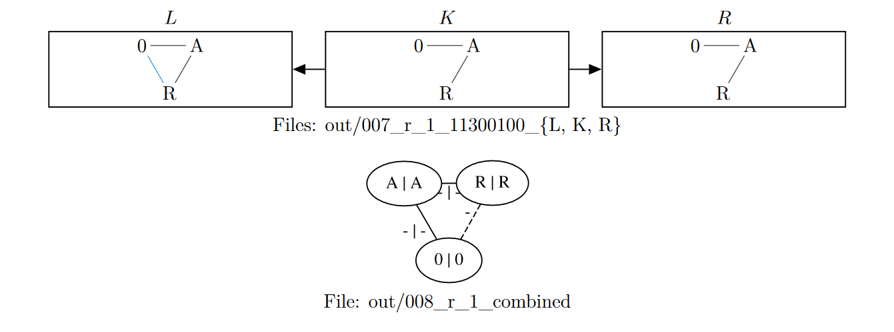
\includegraphics[scale=0.7]{v.png}
\vspace{10mm}

\subsubsection{VI. Unmark collapsed node}

This is 'finishing' rule because it takes the node A upon which we preformed contraction and marks it with 0 again so we could continue with the starting state. Constraint stops that we unmark a central node which has not been collapsed as such node still has nodes marked with R connected to it. Also, there is no need for a context as before application of this rule there should be only one node marked with A on the graph while all others are marked with 0 and we just need to relabel that one node. 

\begin{lstlisting}
rule [
	ruleID "Unmark collapsed node"
	left [
		node [ id 0 label "A" ]
	]
	context [
	]
	right [
		node [ id 0 label "0" ]
	]
	constrainAdj [
		id 0
		op "="
		count 0
		nodeLabels [ label "R" ]
	]
]
\end{lstlisting}

\vspace{10mm}
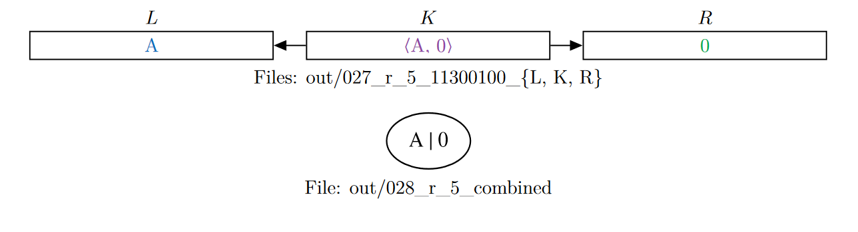
\includegraphics[scale=0.7]{vi.png}
\vspace{10mm}

The main difference in creation of Catalan rules in comparison to Formose and Reindeer is that in previous cases we always had node markings in the context, as the base and on the left and right side there were always bonds which were the only thing that was changing. 

To solve Catalan, different approach should have been used. The first step was to imagine what is each rule supposed to do according to a graph we had and then try to simulate 'movement' in the game by combining them. The first rule, Mark for conversion stands out as a bit different. There we have the total opposite situation from previous two subassignments. In that case, bonds are placed in the context and node labels are the only thing which is changing, so the other rules could be applied to those nodes. The context, left and right side in other five rules cannot be observed in those patterns as they are literally simulating what is stated in their titles.
\\
The way how exactly those rules combined together mimic real Catalan moves together with the flow and the number of steps needed to solve first level are easily visible on the filtered graph. 

\vspace{10mm}
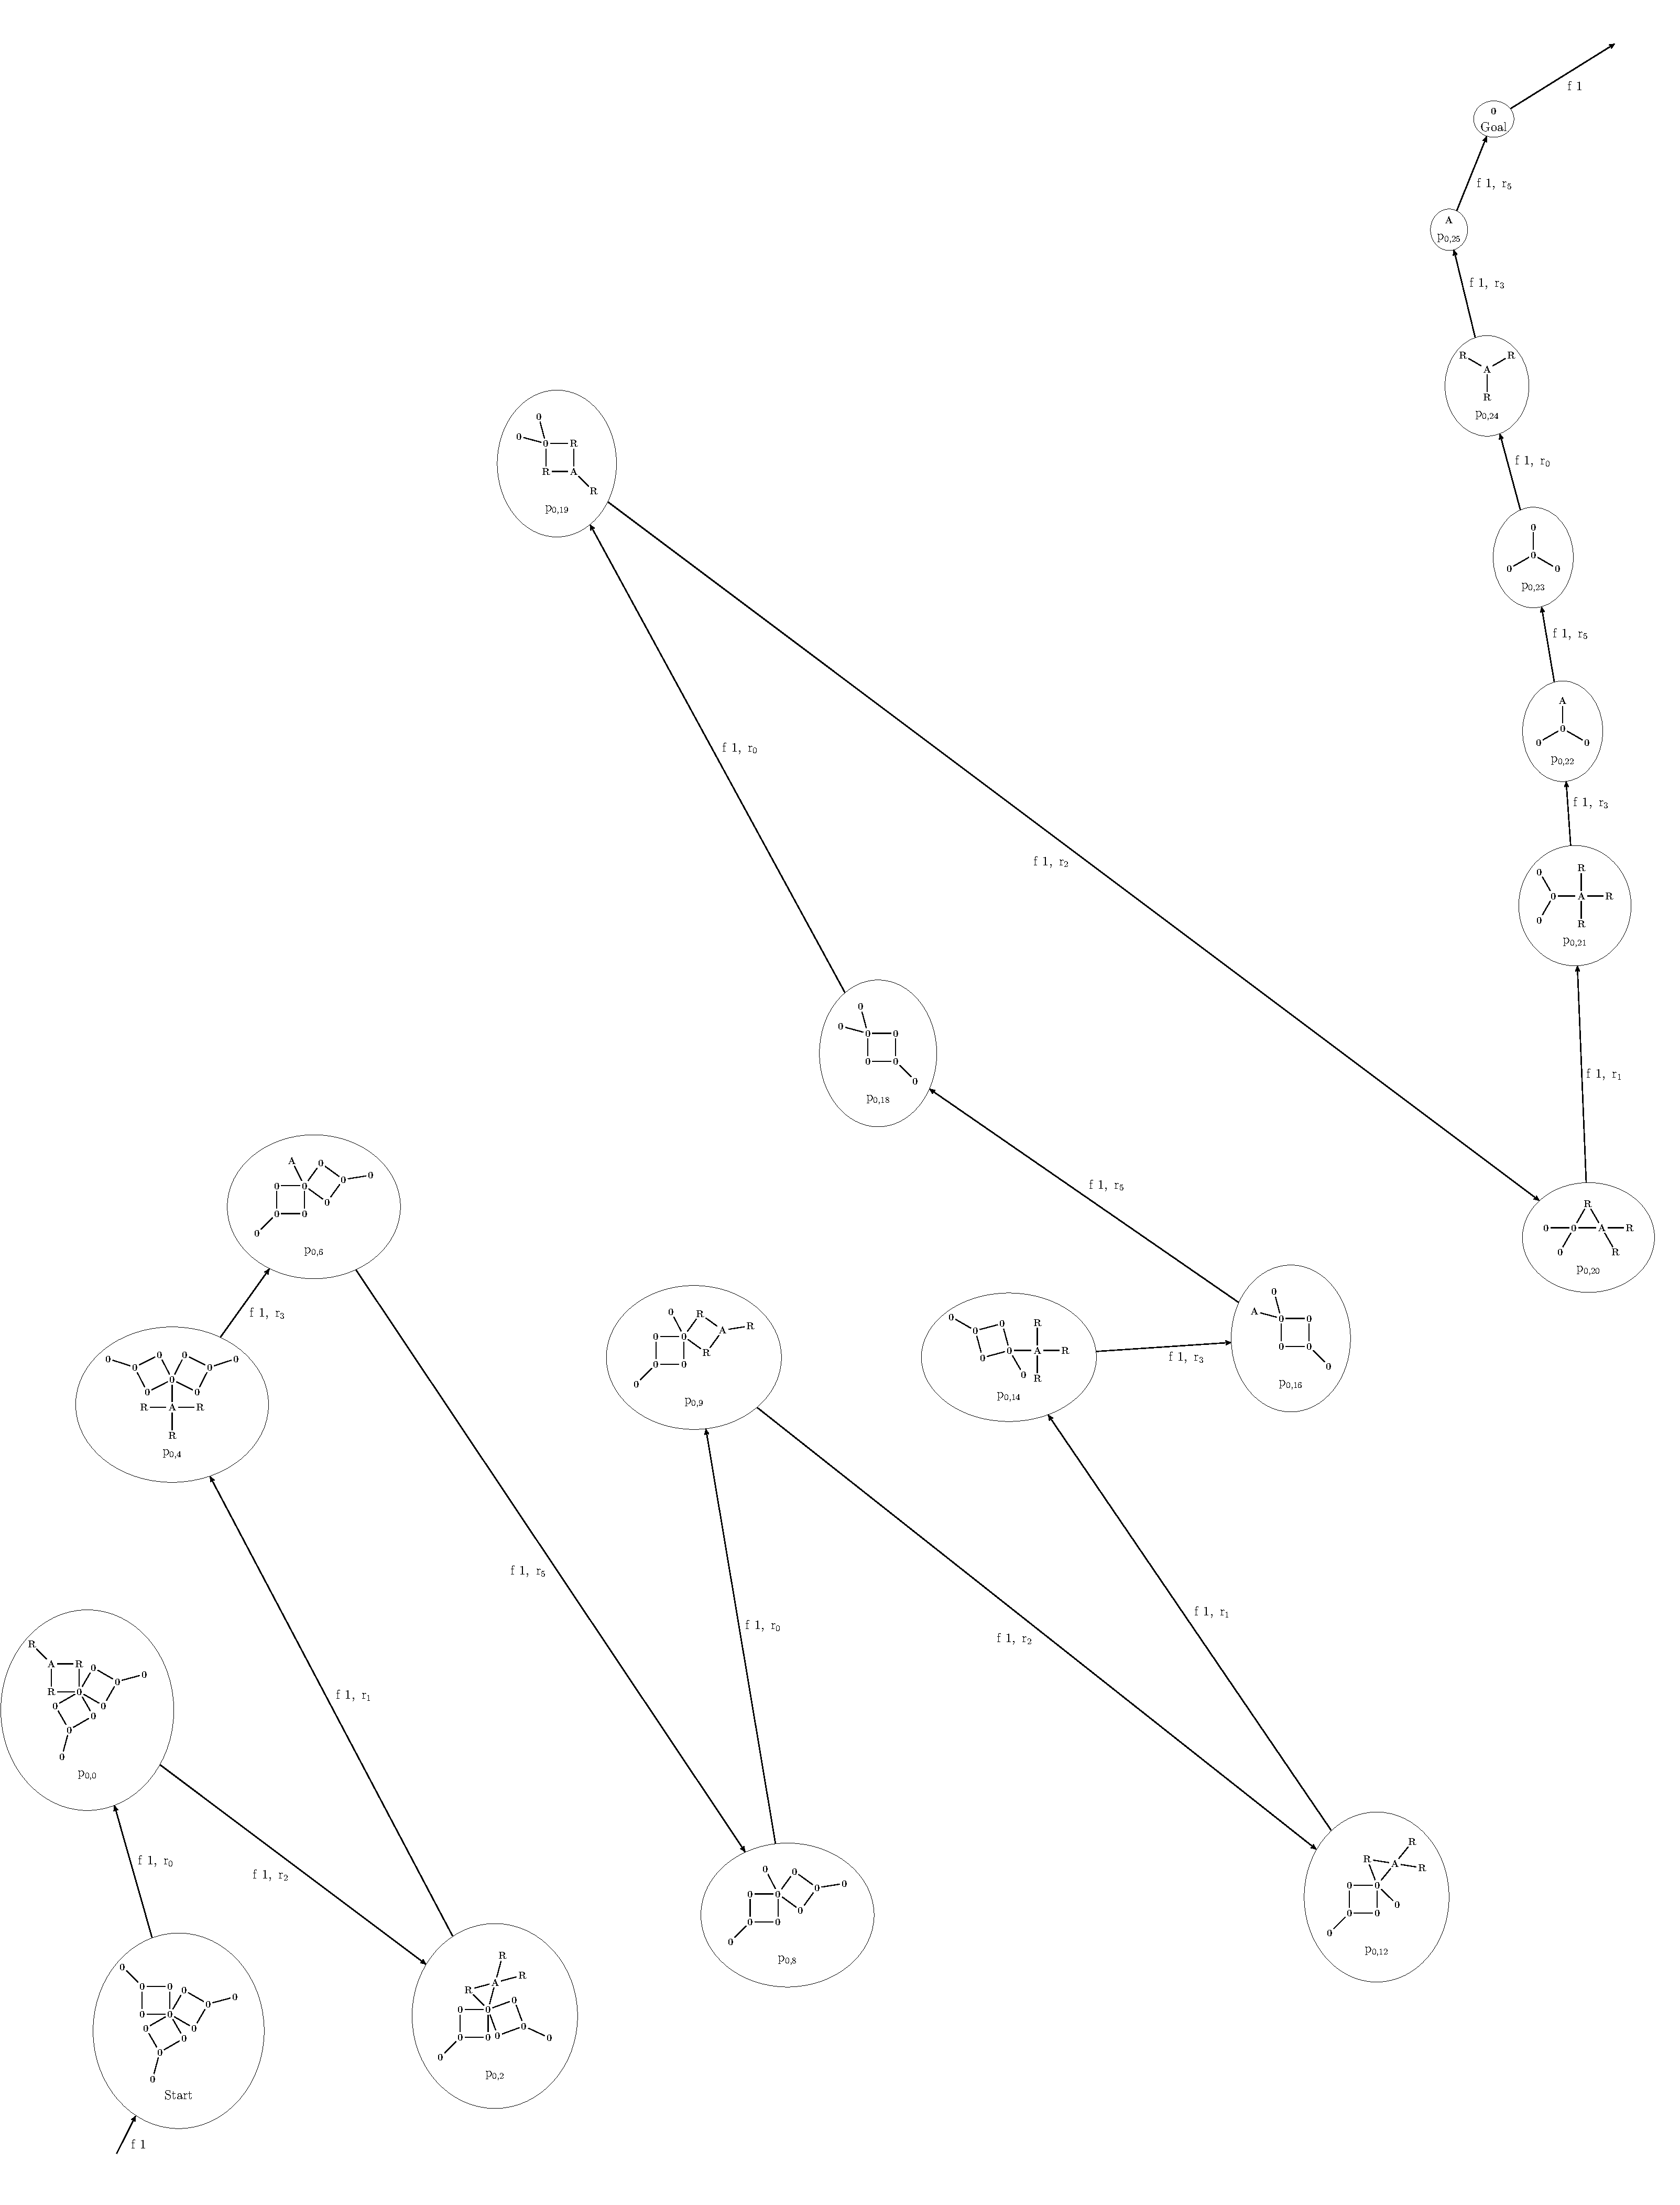
\includegraphics[scale=0.3]{063.pdf}
\vspace{10mm}

Total number of steps to solve the first level is 20 if we count the initial and the final graphs. Appliance of all rules from above is visible, one rule appliance per each step. With graph grammars approach and rules defined as above we were able to solve all catalan levels. 

\newpage
\section{Conclusion}

Doing this project we got a decent understanding of the framework MØD, but there are still a lot of things to learn and concepts to understand.\\
The formose reaction for example currently has a problem, most likely related to the constraints. \\
The reindeer puzzle worked, it was implemented using 14 rules, It could have been done using only 4 if we had used terms but the space would have been huge as everything would have been considered, and not just the limited amount of moves we made available.\\
The catalan game was solved using 6 rules, and a global constraint on A's defined in the python wrapper to reduce the combinatorial mess a bit. More could have been done, but the solution works, it just takes a long time to solve all the levels. It's probably faster to solve them by the hand.
\\
All the summeries and files from the generation can be found at\\
https://imada.sdu.dk/~mjerv15/dm840/assignment1/


\end{document}